%-----------------------------------------------------------------------------
%
%               Template for sigplanconf LaTeX Class
%
% Name:         sigplanconf-template.tex
%
% Purpose:      A template for sigplanconf.cls, which is a LaTeX 2e class
%               file for SIGPLAN conference proceedings.
%
% Guide:        Refer to "Author's Guide to the ACM SIGPLAN Class,"
%               sigplanconf-guide.pdf
%
% Author:       Paul C. Anagnostopoulos
%               Windfall Software
%               978 371-2316
%               paul@windfall.com
%
% Created:      15 February 2005
%
%-----------------------------------------------------------------------------


\documentclass[preprint]{sigplanconf}

% The following \documentclass options may be useful:

% preprint      Remove this option only once the paper is in final form.
% 10pt          To set in 10-point type instead of 9-point.
% 11pt          To set in 11-point type instead of 9-point.
% authoryear    To obtain author/year citation style instead of numeric.

\usepackage{amsmath}
%\usepackage{silence}
\usepackage{pgf}
\usepackage{tikz}
\usetikzlibrary{arrows,automata}
\usepackage{url}
\usepackage[hidelinks]{hyperref}
\usepackage{fancyvrb}
\usepackage[numbers]{natbib}
%\WarningsOff

\newcommand{\useverbtb}[1]{\begin{tiny}\BUseVerbatim{#1}\end{tiny}}
\newcommand{\useverb}[1]{\begin{small}\BUseVerbatim{#1}\end{small}}
\newcommand{\useverbb}[1]{\begin{small}\BUseVerbatim{#1}\end{small}}

\begin{document}
\fvset{fontsize=\small}
\newcommand{\idris}{\textsc{Idris}}
\newcommand{\idata}{\textsf{iData}}
\newcommand{\itasks}{\textsf{iTasks}}
\newcommand{\Idris}{\textsc{Idris}}
\special{papersize=8.5in,11in}
\setlength{\pdfpageheight}{\paperheight}
\setlength{\pdfpagewidth}{\paperwidth}

\conferenceinfo{IFL '13}{August 28--31, 2013, Nijmegen, The Netherlands} 
\copyrightyear{2013} 
\copyrightdata{978-1-nnnn-nnnn-n/yy/mm} 
\doi{nnnnnnn.nnnnnnn}

% Uncomment one of the following two, if you are not going for the 
% traditional copyright transfer agreement.

%\exclusivelicense                % ACM gets exclusive license to publish, 
                                  % you retain copyright

%\permissiontopublish             % ACM gets nonexclusive license to publish
                                  % (paid open-access papers, 
                                  % short abstracts)

\titlebanner{}        % These are ignored unless
\preprintfooter{}   % 'preprint' option specified.

\title{Dependent Types for Safe and Secure Web Programming}
\authorinfo{Simon Fowler \and Edwin Brady}
           {School of Computer Science, University of St Andrews, St Andrews, Scotland}
           {Email: \{sf37, ecb10\}@st-andrews.ac.uk}

\maketitle

\begin{abstract}
Dependently-typed languages allow precise types to be used during development,
facilitating static reasoning about program behaviour. However,
stronger types bring a disadvantage that it becomes increasingly difficult to
write programs that are accepted by a type checker, meaning additional proofs may
have to be specified by a developer.

Embedded domain-specific languages (EDSLs) can help address this problem by
introducing a layer of abstraction over more precise underlying types,
allowing domain-specific code to be written in a high-level language which uses
dependent types to enforce invariants without imposing additional proof
obligations on an application developer. 

In this paper, we apply this technique to web programming.  Using the
dependently typed programming language \Idris{}, we introduce an EDSL to
facilitate the creation and handling of \emph{statically checked} web forms,
reducing the scope for programmer error and attacks such as SQL injection. We
also show how to enforce resource usage protocols associated with common web
operations such as CGI, database access and session handling.  

\end{abstract}

%\category{CR-number}{subcategory}{third-level}

% general terms are not compulsory anymore, 
% you may leave them out
%\terms
%term1, term2

\keywords
Dependent types, web applications, security, verification
%keyword1, keyword2

\section{Introduction}

Web applications, whilst ubiquitous, are also prone to incorrect construction
and security exploits such as SQL injection \cite{owasp:sqli} or cross-site
scripting \cite{owasp:xss}. Security breaches are
far-reaching, and high profile cases involve large corporations such as Sony,
who suffered a well-publicised and extremely costly SQL injection breach in
2011 \cite{ieee:sony}, and \textit{Yahoo!}, who suffered a breach in 2012
\cite{imperva:yahoo}. 

Many web applications are written in dynamically-checked scripting languages
such as PHP, Ruby or Python, which facilitate rapid development
\cite{w3techs:webpls}. Such languages do not, however, provide the same static 
guarantees about runtime behaviour afforded by
programs with more expressive, static type systems, instead relying on
extensive unit testing to ensure correctness and security. 

%%------- EXAMPLE
Let us consider a simple database access routine, written in
PHP, where we wish to obtain the name and address of every employee working in
a given department, \texttt{\$dept}. We firstly construct an object
representing a database connection, where the arguments are the database host,
user, password and name respectively:

\begin{SaveVerbatim}{conn}

$conn = new mysqli("localhost", "username", 
                   "password", "db");

\end{SaveVerbatim}
\useverb{conn}

\noindent
We should then check to see if the connection was successful, and exit
if not:
%This check is optional, so
%it would be possible to omit it. However, this would cause
%problems with later steps.

\begin{SaveVerbatim}{connerr}

if (mysqli_connect_errno()) { exit(); }

\end{SaveVerbatim}
\useverb{connerr}

\noindent
We then create a prepared statement detailing our query, and bind the
\texttt{`dept'} value:

\begin{SaveVerbatim}{prepare}

  $stmt = $conn->prepare("SELECT `name`, `address` 
     FROM `staff` WHERE `dept` = ?);
  $stmt->bind_param('s', $dept);

\end{SaveVerbatim}
\useverb{prepare}

\noindent
After the parameters have been bound, we execute the statement, assign
variables into which results will be stored, and fetch each row in turn. 
Failure to execute a statement before attempting to fetch rows would cause an error, as would attempting to execute a statement without binding variables to it.

\begin{SaveVerbatim}{stmtexec}

$stmt->execute();
$stmt->bind_result($name, $address);
while ($stmt->fetch()) {
  printf("Name: %s, Age: %s", $name, $age);
}

\end{SaveVerbatim}
\useverb{stmtexec}

\noindent
Finally, once the statement and connection are no longer needed, they should be
closed in order to discard the associated resources:

\begin{SaveVerbatim}{connclose}

  $stmt->close();
  $conn->close();

\end{SaveVerbatim}
\useverb{connclose}

\noindent
Even in this small example, there exists a precise resource usage protocol
which must be followed for successful and robust operation.
Firstly, a connection to the database must be opened. The object-oriented style
used in the example encapsulates this to an extent, as the object must be
created in order for operations to be performed, however it is less obvious in
a procedural version of the code. Secondly, a prepared statement is created,
using the raw SQL and placeholders to which variables are later bound. The
statement is then executed, and each row is retrieved from the database.
Finally, the resources are freed. 

Problems may arise if the protocol is not followed correctly.
A developer may, for example, accidentally close a statement whilst still
retrieving rows, which would cause a runtime error. Similarly, a developer may
omit closing the statement or connection, which can lead to
problems such as resource leaks in longer-running server applications.
However, in conventional programming languages, there is no way to check
automatically, at compile-time, that a protocol is followed.

In contrast, the use of \textit{dependent types} makes it possible
to specify a program's behaviour precisely, and to check that a 
specification is followed.
%
Unfortunately, automatic verification by a compiler can be difficult or
often impossible, requiring additional proofs to be given by the developer.

This complexity can be addressed through the use of \textit{embedded
domain-specific languages} (EDSLs) to abstract away the complexity of the
underlying type system. Embedding a domain-specific language in
a dependently typed host language
allows domain experts to write 
domain-specific code, with the EDSL itself used to provide the proof that the
code is correct.

\idris{} \cite{brady2013idris} is a language with full dependent types, and
extensive support for EDSLs through overloading and syntax macros. Through the
use of \idris{}, and a framework for describing resource protocols using
\emph{algebraic effects}~\cite{brady:effects}, we
present a dependently-typed web framework allowing the construction of
programs with additional guarantees about correctness and security, whilst
minimising the increase in development complexity. 

\subsection{Contributions}
The primary contribution of this paper is the application of 
dependent types to provide strong static guarantees
about the correctness and security of web applications, whilst minimising
additional development complexity. In particular, we present:

\begin{itemize}
\item Representations of CGI, Databases and sessions as
\textit{resource-dependent algebraic effects}, allowing programs to be accepted
only when they follow clearly defined resource usage protocols. 
(Section~\ref{rup})

\item Type-safe form handling, preserving type information and managing
user input, therefore increasing applications' resilience to attacks such as
SQL injection and cross-site scripting. (Section~\ref{form})

\item An extended example: a message board application, demonstrating the usage
of the framework in practice. (Section~\ref{effects})

\end{itemize}

We achieve these without extending the host language. Every
resource protocol we implement is pure \Idris{}, using a library for
resource-dependent algebraic effects~\cite{brady:effects} and \Idris{}'
features for supporting domain-specific language implementation such as
syntax macros and overloading. In particular, this means the same techniques
can be applied to other resources, and most importantly, combinations
of resources and DSLs implemented in this way are \emph{composable}.

%We structure the remainder of this paper as follows. We provide a brief
%overview of the \texttt{Effects} framework in Section ~\ref{effects}; explain
%how this may be used to ensure adherence to resource usage protocols for CGI,
%SQLite and a session handler in Section ~\ref{rup}; describe an EDSL for
%type-safe form handling in Section ~\ref{form}, implemented using
%\texttt{Effects}; and discuss the larger example
%of a message board system making use of these components in Section
%~\ref{messageboard}.

The code used to implement the framework and all associated examples used in
this paper is available online at
\url{http://www.github.com/idris-hackers/IdrisWeb}.

% =================================================
% =================================================
\section{An overview of the \texttt{Effects} framework}
\label{effects}

\texttt{Effects}~\cite{brady:effects} is an \idris{} library which handles
side-effects such as state, exceptions, and I/O as \emph{algebraic
effects}~\cite{Plotkin2009}. In particular, it supports parameterising effects
by an input and output \emph{state}, which permits effectful programs to track
the progress of a resource usage protocol. Effectful programs are written
in a monadic style, with \texttt{do}-notation, with their type stating which
specific effects are available.
Effectful
programs are described using the following data type,
in the simplest case:

\begin{SaveVerbatim}{efftype}

Eff : (m : Type -> Type) ->
      (es : List EFFECT) -> (a : Type) -> Type

\end{SaveVerbatim}
\useverb{efftype}

\noindent
\texttt{Eff} is parameterised over a \emph{computation context}, \texttt{m}, 
which describes the context in which the effectful program will be run, a
list of side effects \texttt{es} that the program is permitted to use, and the
program'’s return type \texttt{a}. The name \texttt{m} for the computation context is
suggestive of a monad, but there is no requirement for it to be so.

For example, the following type carries an integer state,
throws an exception of type \texttt{String} if the state reaches 100, 
and runs in a \texttt{Maybe} context:

\begin{SaveVerbatim}{addState}

addState : Eff Maybe [STATE Int, EXCEPTION String] ()
addState = do val <- get
              when (val == 100) (raise "State too big")
              put (val + 1)

\end{SaveVerbatim}
\useverb{addState}

\subsection{Implementing Effects}

Effects such as `State' and `Exception' are described as algebraic data types,
and run by giving \emph{handlers} for specific computation contexts. 
Effects have a corresponding \emph{resource} (in the case of state, the
resource is simply the current state). Executing an effectful operation may
change the resource and return a value:

\begin{SaveVerbatim}{efffam}

Effect : Type
Effect = (in_res : Type) -> (out_res : Type) -> 
         (val : Type) -> Type

\end{SaveVerbatim}
\useverb{efffam}

\noindent
For example, the state effect is described as follows:

\begin{SaveVerbatim}{stateeff}

data State : Effect where
     Get :      State a a a
     Put : b -> State a b ()

\end{SaveVerbatim}
\useverb{stateeff}

\noindent
That is, \texttt{Get} returns a value of type \texttt{a} without updating
the resource type. \texttt{Put} returns nothing, but has the effect of updating
the resource. To make an effect usable, we implement a handler
for a computation context by making an instance of the following class:

\begin{SaveVerbatim}{effhandler}

class Handler (e : Effect) (m : Type -> Type) where
     handle : res -> (eff : e res res' t) -> 
              (k: res' -> t -> m a) -> m a

\end{SaveVerbatim}
\useverb{effhandler}

\noindent
The \texttt{handle} function takes the input resource, an effect which may
update that resource and execute a side-effect, and a continuation \texttt{k}
which takes the updated resource and the return value of the effect. We use
a continuation here primarily because there is no restriction on the number of
times a handler may invoke the continuation (raising an exception, for example,
will not invoke it). Reading and updating states is handled
for all computation contexts \texttt{m}:

\begin{SaveVerbatim}{statehandler}

instance Handler State m where
     handle st Get     k = k st st
     handle st (Put n) k = k n ()

\end{SaveVerbatim}
\useverb{statehandler}

\noindent
Finally, we promote \texttt{State} into a concrete effect \texttt{STATE}, and
the \texttt{Get} and \texttt{Put} operations into functions in \texttt{Eff}, as
follows:

\begin{SaveVerbatim}{stateconc}

STATE : Type -> EFFECT
STATE t = MkEff t State

get : Eff m [STATE x] x
get = Get 

put : x -> Eff m [STATE x] ()
put val = Put val

\end{SaveVerbatim}
\useverb{stateconc}

\noindent
A concrete effect is simply an algebraic effect type paired with its current
resource type. This, and other
technical details, are explained in full elsewhere~\cite{brady:effects}.
For the purposes of this paper, it suffices to know how to describe and
handle new algebraic effects.

\subsection{Resource Protocols as Effects}

\begin{SaveVerbatim}{fileeff}
{-                                             { Input resource type }   { Output resource type } { Value } -}
 
data FileIO : Effect where
     Open      : String -> (m : Mode) -> FileIO     ()                    (Either () (OpenFile m)) ()
     Close     :                         FileIO     (OpenFile m)          ()                       ()

     ReadLine  :                         FileIO     (OpenFile Read)       (OpenFile Read)          String
     WriteLine : String ->               FileIO     (OpenFile Write)      (OpenFile Write)         ()
     EOF       :                         FileIO     (OpenFile Read)       (OpenFile Read)          Bool
\end{SaveVerbatim}

\begin{figure*}[t]
\begin{center}
\useverb{fileeff}
\end{center}
\caption{File Protocol Effect}
\label{fig:fileeffect}
\end{figure*}
More generally, a program might modify the set of effects available.
This might be desirable for several reasons, such as adding a new
effect, or to update an index of a dependently typed state. In this
case, we describe programs using the \texttt{EffM} data type:

\begin{SaveVerbatim}{effmtype}

EffM : (m : Type -> Type) ->
       (es : List EFFECT) -> (es' : List EFFECT) ->
       (a : Type) -> Type

\end{SaveVerbatim}
\useverb{effmtype}

\noindent
\texttt{EffM} is parameterised over the context and type as before, but
separates input effects (\texttt{es}) from output effects (\texttt{es'}). 
In fact, \texttt{Eff}
is defined in terms of \texttt{EffM}, with equal input/output effects.
We can use this to describe how effects follow resource protocols. A simple
example is a file access protocol, where a file must be opened before it
is read or written, and a file must be closed on exit. 

Figure \ref{fig:fileeffect} shows how the protocol is encoded as an
effect.
Note that the types of the input and output resources describes how resource
state changes in each operation: opening a file may fail, so
changes an empty resource to
a resource containing either a unit or an open file; 
reading a line is only possible if the
resource is a file open for reading, etc.
The handler for this effect for an \texttt{IO} computation context will
execute the required primitive I/O actions.

The following program type checks, and therefore implicitly carries 
a proof that the file resource protocol is followed correctly:

\begin{SaveVerbatim}{testfile}

testFile : Eff IO [FILE_IO (), STDIO] () 
testFile = do open "testFile" Read
              if_valid then do str <- readLine
                            close
                            putStrLn str
                       else putStrLn "Error"

\end{SaveVerbatim}
\useverb{testfile}

\noindent
The type of \texttt{testFile} states
that File I/O and console I/O are available effects, and in particular that
the resource associated with the File I/O will be in the same state on entry
and exit. We use \texttt{if\_valid} to handle possible failure---this is
a function provided by the \texttt{Effects} library which checks whether
a resource of type \texttt{Either a b} indicates failure (\texttt{Left a})
or success (\texttt{Right b}). In this case, the initial resource in the valid
branch is \texttt{OpenFile Read}, indicating that the file has been successfully 
opened for reading, whereas in the failing branch, the resource remains as \texttt{()}.

Attempting to write to the file, failing to check for
success, or failing to open or close the
file, would cause a \emph{compile-time} error. 

We will use this technique extensively
throughout this paper: describe a resource usage protocol in terms of
state transitions; implement an effect which captures that protocol; and implement
programs which, by using this effect, implicitly carry a proof that the resource
protocol has been correctly followed.


% =================================================
% =================================================
\section{Modelling resource usage protocols}
\label{rup}
In this section, we show how three effects 
(CGI, database access and a simple session handler) may be implemented, and
describe the benefits of developing programs using this technique over simply
handling them in \texttt{IO} or as monad transformers.

% =================================================

\subsection{CGI}
%TODO: Fix up the labels
\begin{figure}[htpb!]
\centering
\scalebox{0.8}{
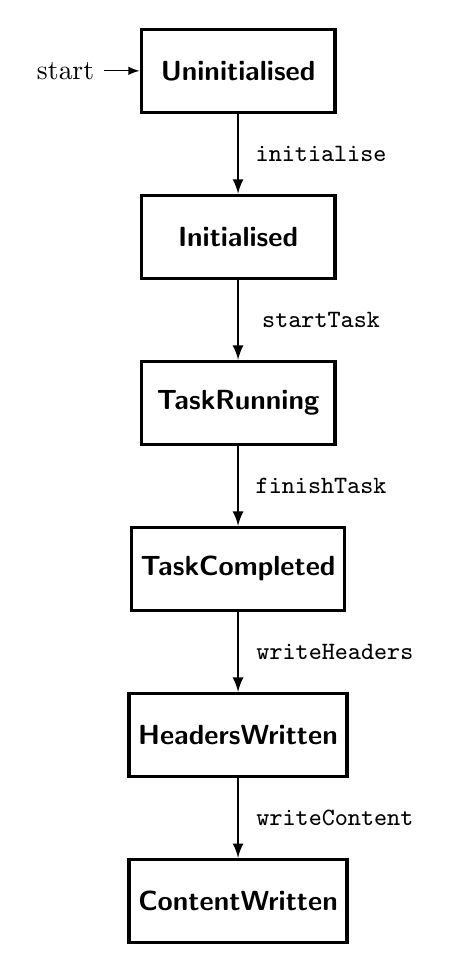
\begin{tikzpicture}[>=latex]
  \tikzstyle{state} = [draw, very thick, fill=white, rectangle, minimum height=3em, minimum width=7em, node distance=6em, font={\sffamily\bfseries}]
  
  \tikzstyle{stateEdgePortion} = [black,thick];
  \tikzstyle{stateEdge} = [stateEdgePortion,->];
  \tikzstyle{edgeLabel} = [pos=0.5, font={\sffamily\small}];

  \node[initial,state] (A)              {Uninitialised};
  \node[state]         (B) [below of=A] {Initialised};
  \node[state]         (C) [below of=B] {TaskRunning};
  \node[state]         (D) [below of=C] {TaskCompleted};
  \node[state]         (E) [below of=D] {HeadersWritten};
  \node[state]         (F) [below of=E] {ContentWritten};

  \path (A) edge[stateEdge]   node[edgeLabel, xshift=3em] {\texttt{initialise}} (B)
        (B) edge[stateEdge]   node[edgeLabel, xshift=3em] {\texttt{startTask}} (C)
        (C) edge[stateEdge]   node[edgeLabel, xshift=3em] {\texttt{finishTask}} (D)
        (D) edge[stateEdge]   node[edgeLabel, xshift=3.5em] {\texttt{writeHeaders}} (E)
        (E) edge[stateEdge]   node[edgeLabel, xshift=3.5em] {\texttt{writeContent}} (F);
\end{tikzpicture}
}
\caption{CGI States}
\label{fig:cgistates}
\end{figure}

CGI is used to invoke an application on a web server, making use of environment
variables to convey information gained from an HTTP request and using standard
output to communicate with the remote client. Importantly, HTTP headers must be
correctly written to the browser prior to any other output; failure to do so
will result in an internal server error being shown.

By modelling CGI as a resource-dependent algebraic effect, we may enforce a
resource usage protocol which
prevents arbitrary IO from being performed and therefore
ensures that the headers are written correctly. We
define an effect, \texttt{Cgi}, and an associated resource,
\texttt{InitialisedCGI}, parameterised over the current state,
\texttt{CGIStep}, and containing a
\texttt{CGIInfo} record which contains information from the request. We
represent an uninitialised CGI process as the unit type, \texttt{()}.

\begin{SaveVerbatim}{cgistep}

data CGIStep = Initialised   | TaskRunning 
             | TaskCompleted | HeadersWritten 
             | ContentWritten

data InitialisedCGI : CGIStep -> Type where
     ICgi : CGIInfo -> InitialisedCGI s

\end{SaveVerbatim}
\useverb{cgistep}

\noindent
Figure~\ref{fig:cgistates} shows the states through which the CGI program
progresses, and Figure~\ref{fig:cgieffect} shows how this is represented
as a resource-dependent algebraic effect. Each operation performed in an effectful
program requires the resource to be of a certain type, and the completion of
the operation may alter the type or value of the resource. The \texttt{Cgi}
effect declaration shows these resource updates in the types of each operation,
effectively specifying a state machine.

Upon creation, the CGI application is uninitialised, meaning that environment variables have not been queried to populate the CGI state. The only operation
that can be performed in this state is initialisation: by calling
\texttt{initialise}, a \texttt{CGIInfo} record is populated, and the state transitions
to \texttt{Initialised}. The \texttt{Init} operation is defined as part of the
\texttt{Cgi} effect, and involves transitioning from the uninitialised state to
the initialised state.

\begin{SaveVerbatim}{cgieff}
{-                     { Input resource type }         { Output resource type }        { Value } -}

data Cgi : Effect where
    Init         : Cgi ()                              (InitialisedCGI Initialised)    ()
    StartRun     : Cgi (InitialisedCGI Initialised)    (InitialisedCGI TaskRunning)    ()
    FinishRun    : Cgi (InitialisedCGI TaskRunning)    (InitialisedCGI TaskCompleted)  ()
    WriteHeaders : Cgi (InitialisedCGI TaskCompleted)  (InitialisedCGI HeadersWritten) ()
    WriteContent : Cgi (InitialisedCGI HeadersWritten) (InitialisedCGI ContentWritten) ()
    OutputData   : String -> 
                   Cgi (InitialisedCGI TaskRunning)    (InitialisedCGI TaskRunning)    ()
    RunAction    : Env IO (CGI (InitialisedCGI TaskRunning) :: effs) -> CGIProg effs a -> 
                   Cgi (InitialisedCGI TaskRunning)    (InitialisedCGI TaskRunning)    a
\end{SaveVerbatim}

\begin{figure*}[t]
\begin{center}
\useverb{cgieff}
\end{center}
\caption{CGI Effect}
\label{fig:cgieffect}
\end{figure*}

Additional operations, including those to query \texttt{POST} and \texttt{GET}
variables, are omitted in the interest of brevity.

User code executes in the \texttt{TaskRunning} state. Several operations, such
as querying the \texttt{POST} and \texttt{GET} variables, are available in this state, alongside
functions to output data to the web page and append data to the response
headers. It is important to note that at this stage nothing is written to the
page, with the \texttt{output} and \texttt{addHeader} functions instead
modifying the \texttt{CGIInfo} record. This data may then be printed at the end of the
program's execution, in accordance with the resource usage protocol.

After the user code has finished execution, control returns to the library
code. At this point, the state transitions to TaskCompleted, and the headers
are written.  Finally, the headers and content are written which completes the
process. Since we parameterise the resource over a state, we may ensure that
certain operations only happen in a particular prescribed order.

In \idris{}, types are first-class, meaning that they may be treated like other
terms in computations. We may therefore define the following type synonym, used
within the CGI section of the framework to denote an effectful CGI program: 

\begin{SaveVerbatim}{cgiprog}

CGIProg : List EFFECT -> Type -> Type
CGIProg effs a = 
  Eff IO (CGI (InitialisedCGI TaskRunning) :: effs) a

\end{SaveVerbatim}
\useverb{cgiprog}

\noindent
This is then passed, along with initial values for other effects that the user
may wish to use, to the runAction function, which invokes the RunAction
operation and executes the user-specified action.
%
A simple ``Hello, world!'' program would be defined as follows:

\begin{SaveVerbatim}{hworldcgi}

module Main
import Cgi

sayHello : CGIProg [] ()
sayHello = output "Hello, world!"

main : IO ()
main = runCGI [initCGIState] sayHello

\end{SaveVerbatim}
\useverb{hworldcgi}
% =================================================

Here, \texttt{output} is a function which appends some output to the CGI output buffer, which is later written to the page.

\subsection{Database access with SQLite}

SQLite\footnote{\texttt{http://www.sqlite.org}} is a lightweight SQL database
engine often used as simple, structured storage for larger applications. We
make use of SQLite to demonstrate a resource usage protocol for database access due to its simplicity, although we envisage that these
concepts would be applicable to more complex database management systems. 

The creation, preparation and execution of SQL queries has a specific usage
protocol, with several possible points of failure. Failure is handled in
traditional web applications by the generation of exceptions, which may be
handled in the program.  Handling such exceptions is often optional, however,
and in some cases unhandled errors may cause a deployed web application to
display an error to the user. Such errors can be used to determine the
structure of an insecure SQL query, and are often used by attackers to
determine attack vectors for SQL injection attacks.

\begin{SaveVerbatim}{databaseeff}
{-                           { Input resource type }    { Output resource type }             { Value }           -}
data Sqlite : Effect where
  OpenDB            : DBName -> 
                      Sqlite ()                         (Either () SQLiteConnected)          (Either SQLiteCode ())
  CloseDB           : Sqlite (SQLiteConnected)          ()                                   ()
  PrepareStatement  : QueryString -> 
                      Sqlite (SQLiteConnected)          (Either (SQLitePSFail) 
                                                          (SQLitePSSuccess Binding))         (Either SQLiteCode ())
  BindInt           : ArgPos -> Int -> 
                      Sqlite (SQLitePSSuccess Binding)  (SQLitePSSuccess Binding)            ()
  FinishBind        : Sqlite (SQLitePSSuccess Binding)  (Either SQLiteFinishBindFail
                                                          (SQLitePSSuccess Bound))           (Maybe BindError)
  ExecuteStatement  : Sqlite (SQLitePSSuccess Bound)    (Either (SQLiteExecuting InvalidRow)
                                                          (SQLiteExecuting ValidRow)         StepResult
  RowStep           : Sqlite (SQLiteExecuting ValidRow) (Either (SQLiteExecuting InvalidRow)
                                                          (SQLiteExecuting ValidRow))        StepResult
  GetColumnText     : Column -> 
                      Sqlite (SQLiteExecuting ValidRow) (SQLiteExecuting ValidRow)           String
                      
  CleanupPSFail     : Sqlite (SQLitePSFail)             ()                                   ()
  CleanupBindFail   : Sqlite (SQLiteFinishBindFail)     ()                                   ()

\end{SaveVerbatim}

\begin{figure*}[t]
\begin{center}
\useverb{databaseeff}
\end{center}
\caption{Database Effect}
\label{fig:dbeffect}
\end{figure*}

%TODO: Fix up the labels
\begin{figure}
\centering
\scalebox{0.8}{
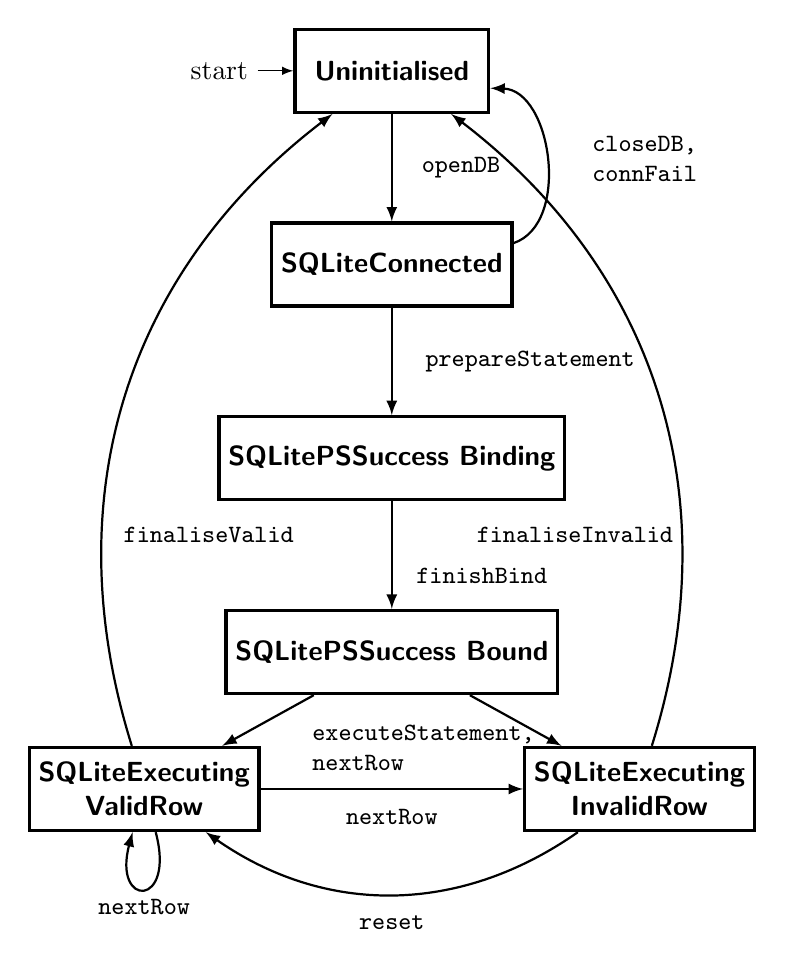
\begin{tikzpicture}[>=latex]
  \tikzset{every loop/.style={min distance=10mm,looseness=5}}
  \tikzstyle{state} = [draw, very thick, fill=white, rectangle, minimum height=3em, minimum width=7em, align=center, node distance=7em, font={\sffamily\bfseries}]
  
  \tikzstyle{stateEdgePortion} = [black,thick];
  \tikzstyle{stateEdge} = [stateEdgePortion,->];
  \tikzstyle{edgeLabel} = [pos=0.5, font={\sffamily\small}];

  \node[initial,state] (A)              {Uninitialised};
  \node[state]         (B) [below of=A] {SQLiteConnected};
  \node[state]         (C) [below of=B] {SQLitePSSuccess Binding};
  \node[state]         (D) [below of=C] {SQLitePSSuccess Bound};
  \node[state]         (E) [below left of=D, xshift=-4em] {SQLiteExecuting \\ ValidRow};
  \node[state]         (F) [below right of=D, xshift=4em] {SQLiteExecuting \\ InvalidRow};

  \path (A) edge[stateEdge]   node[edgeLabel, xshift=2.5em] {\texttt{openDB}} (B)
        (B) edge[stateEdge, bend right=80]   node[edgeLabel, text width=2cm, xshift=4.5em] {\texttt{closeDB, connFail}} (A)
        (B) edge[stateEdge]   node[edgeLabel, xshift=5em] {\texttt{prepareStatement}} (C)
        (C) edge[stateEdge]   node[edgeLabel, xshift=3.25em, yshift=-0.75em] {\texttt{finishBind}} (D)
        (D) edge[stateEdge]   node[edgeLabel, text width=2cm, xshift=-4.5em, yshift=-1em] {\texttt{executeStatement, nextRow}} (F)
        (D) edge[stateEdge]   node[edgeLabel, xshift=3em] {} (E)
        (E) edge[stateEdge, bend left=35]   node[edgeLabel, xshift=3em, yshift=-5em] {\texttt{finaliseValid}} (A)
        (F) edge[stateEdge, bend right=35]   node[edgeLabel, xshift=-3em, yshift=-5em] {\texttt{finaliseInvalid}} (A)
        (E) edge[stateEdge]   node[edgeLabel, yshift=-1em] {\texttt{nextRow}} (F)
        (F) edge[stateEdge, bend left=35]   node[edgeLabel, yshift=-1em] {\texttt{reset}} (E)
        (E) edge[stateEdge, loop below]   node[edgeLabel] {\texttt{nextRow}} (E);
        
\end{tikzpicture}
}
\caption{Database Resource Usage Protocol}
\label{fig:sqlitestates}
\end{figure}

Figure~\ref{fig:sqlitestates} shows a resource usage protocol for database
access, which we have implemented for the SQLite library. Although some
additional states are used to capture failing computations, these are omitted
from the diagram.
The effect implementation is given in Figure \ref{fig:dbeffect}.
%
There are three main phases involved in the usage of the SQLite protocol:
connection to the database, preparation of a query, and execution of the query.
We define several resources to encapsulate the state at any given point during the protocol.

We first define the \texttt{SQLiteConnected} resource, which signifies that a
successful connection has been made to the database. This resource contains a
pointer to the database structure which is used in further computations.

\begin{SaveVerbatim}{sqliteconnected}

data SQLiteConnected : Type where
  SQLConnection : ConnectionPtr -> SQLiteConnected
  
\end{SaveVerbatim}  
\useverb{sqliteconnected}

\noindent
We secondly define resource types to capture success and failure states
of binding a prepared statement:
\texttt{SQLitePSSuccess}, 
\texttt{SQLitePSFail}, and \texttt{SQLiteFinishBindFail}. The types are
declared as follows (we leave the definitions abstract):

\begin{SaveVerbatim}{sqliteconnected}

data BindStep = Binding | Bound
data SQLitePSSuccess : BindStep -> Type where
data SQLitePSFail : Type where
data SQLiteFinishBindFail : Type where

\end{SaveVerbatim}

%  SQLitePS       : ConnectionPtr -> 
%                   StmtPtr -> SQLitePSSuccess a
%  SQLiteBindFail : ConnectionPtr -> 
%                   StmtPtr -> 
%                   BindError -> SQLitePSSuccess a
%data SQLitePSFail : Type where
%  PSFail : ConnectionPtr -> SQLitePSFail
%
%data SQLiteFinishBindFail : Type where
%  SQLiteFBFail : ConnectionPtr -> StmtPtr -> 
%                 SQLiteFinishBindFail

\useverb{sqliteconnected}

\noindent
The \texttt{SQLitePSSuccess} resource indicates that a prepared statement has been correctly created by the underlying library, given a query string. The resource is parameterised by the \texttt{BindStep} type, which indicates whether the binding process has been completed. Should the creation of a prepared statement fail, the resource will be set to \texttt{SQLitePSFail}. 

%To avoid having to explicitly check for failures each time a variable is bound to an argument in the prepared statement, any failures are recorded by constructing the resource with the \texttt{SQLiteBindFail} constructor. Should any binding operations be called whilst in this state, the operations will not be passed to the underlying library. After the binding stage has completed, the \texttt{FinishBind} operation is called. This operation inspects the resource and either transitions to the \texttt{SQLitePSSuccess Bound} state, indicating that all bind operations were successful, or to the \texttt{SQLiteFinishBindFail} state, should a binding operation have been unsuccessful. 

SQLite operates by loading database rows into a buffer, the contents of which may then be accessed through several column access functions. After all rows returned by a query have been processed, no further calls to fetch more rows may be made. Additionally, no calls to column access functions may be made whilst there is no row being currently processed. 

Through the use of dependent types, we may encode these invariants statically, using the \texttt{SQLiteExecuting} resource. This is parameterised by the \texttt{ExecutionResult} data type, which indicates whether there is currently a valid row in the buffer.

\begin{SaveVerbatim}{sqliteexecuting}

data ExecutionResult = ValidRow
                     | InvalidRow

data SQLiteExecuting : ExecutionResult -> Type where
  SQLiteE : ConnectionPtr -> 
            StmtPtr -> SQLiteExecuting a
  
\end{SaveVerbatim}
\useverb{sqliteexecuting}
\noindent
Column access functions may only be called when there is a valid row in the
buffer, as signified by the input resources:

\begin{SaveVerbatim}{getcoltext}

GetColumnText : Column -> 
                Sqlite (SQLiteExecuting ValidRow) 
                       (SQLiteExecuting ValidRow)
                       String
                         
\end{SaveVerbatim}
\useverb{getcoltext}

\noindent
In order to provide the necessary static guarantee that there is a valid row to
process in the buffer, we make use of the \texttt{if\_valid} construct. The
\texttt{nextRow} function will either fetch a row into the buffer, or indicate
that a row could not be loaded, as shown by its type:

\noindent
\begin{SaveVerbatim}{nextrow}

nextRow : EffM IO [SQLITE (SQLiteExecuting ValidRow)] 
         [SQLITE (Either (SQLiteExecuting InvalidRow)
                 (SQLiteExecuting ValidRow))] StepResult

\end{SaveVerbatim}
\useverb{nextrow}

\noindent
The \texttt{if\_valid} construct provides failure checking functionality, allowing different operations to be performed depending on whether or not a row was successfully fetched for processing.
%If a failure happens at any point during the computation, the resource is
%updated to reflect the failure: if, for example, the library failed to create a
%connection to the database, the resource value would be updated to
%\texttt{OpenConn InvalidConn}. At this point, no further side-effecting
%requests are made to the underlying SQLite library, in order to ensure safety.
%The \texttt{connFail}, \texttt{stmtFail}, \texttt{bindFail} and
%\texttt{executeFail} utility functions allow for failures, once detected, to be
%handled by executing the appropriate sequence of state transition functions to
%dispose of any open resources and return to the initial protocol state. 

%Queries are evaluated through one or more calls to the \texttt{nextRow} function, which either executes an update statement or returns the next row of a result set. 
%SQL queries are evaluated in SQLite upon a call to the C library function
%\texttt{sqlite3\_step()}. In the case that a statement returns a result set,
%each subsequent call retrieves another row for processing using a column access
%function. Once all rows have been retrieved, the library returns
%\texttt{SQLITE\_DONE}, meaning that no further calls should be made without
%resetting the function. We encapsulate this requirement through the
%\texttt{StepResult} data type within the \texttt{ExecutingStmt} constructor. 

%\begin{SaveVerbatim}{stepres}

%data StepResult = Unstarted    | StepFail
%                | StepComplete | NoMoreRows

%\end{SaveVerbatim}
%\useverb{stepres}

By incorporating pointers to open connections and prepared statements into the
resource associated with the effect, we introduce a further layer of
abstraction, which hides implementation details from the developer and
encourages less error-prone code. 

\subsubsection{Example}

%Programs making use of the DSL should look familiar to developers even without
%a background in functional programming. 
To demonstrate the 
library, we return to the previous example of selecting the names and addresses
of all staff working in a given department. 
%Since the
%\texttt{Effects} library overloads the bind operator, we may make use of
%\texttt{do}-notation, facilitating the usage of an imperative style.
We define a function \texttt{textSel} of type:

\noindent
\begin{SaveVerbatim}{sqleffty}

String -> Eff IO [SQLITE ()] 
           (Either QueryError (List (String, String)))

\end{SaveVerbatim}
\useverb{sqleffty}

\noindent
The program will be run in \texttt{IO}, and starts and finishes with no active
resources.  It returns either a list of \texttt{(String, String)} pairs,
representing names and addresses in the database, or an error.
%This example is shown in Figure
%\ref{fig:testsel}.

\begin{SaveVerbatim}{testsel}
testSelect : String -> Eff IO [SQLITE ()] 
             (Either QueryError (List (String, String)))
testSelect dept = do
  db_res <- openDB "people.db"
  if_valid then do
    let sql = "SELECT name, address FROM `staff` 
                    WHERE dept = ?;"
    sql_prep_res <- prepareStatement sql
    if_valid then do 
      bindText 1 dept
      bind_res <- finishBind
      if_valid then do
        executeStatement
        results <- collectResults
        finaliseInvalid
        closeDB
        Effects.pure $ Right results
      else do
        cleanupBindFail
        Effects.pure $ Left (getBindError bind_res)
    else do
      cleanupPSFail
      Left $ getQueryError sql_prep_res
  else do 
    Effects.pure $ Left (getQueryError db_res)
\end{SaveVerbatim}

\begin{figure}[h]
\useverb{testsel}
\caption{Example SQL program}
\label{fig:testsel}
\end{figure}

The program initially attempts to open a connection to the \texttt{people.db}
database. At this point, since the \texttt{OpenDB} operation has been invoked,
the program transitions to the \texttt{ConnectionOpened} state. The
\texttt{openDB} function returns either an error code, if the connection fails, or a unit type should the connection succeed, as shown in Figure \ref{fig:sqlitestates}.

A call to \texttt{prepareStatement} attempts to create a prepared statement,
and a subsequent call to \texttt{beginExecution} allows data to be retrieved
from the database.
%
\texttt{CollectResults} operates on the row currently held in the buffer.
Firstly, the function checks
that there is a valid row in the buffer, and if so uses the
\texttt{getColumnText} function to retrieve the data
from the database. This function is then called recursively until there are no
more rows to process.

\begin{SaveVerbatim}{collectresty}

collectResults :
  EffM IO [SQLITE (Either (SQLiteExecuting InvalidRow) 
                          (SQLiteExecuting ValidRow))] 
          [SQLITE (SQLiteExecuting InvalidRow)] 
          (List (String, String))
\end{SaveVerbatim}

\begin{SaveVerbatim}{collectres}
collectResults = 
  if_valid then do name <- getColumnText 1
                   addr <- getColumnText 2
                   step_res <- nextRow
                   xs <- collectResults
                   return $ (name, addr) :: xs
  else return []

\end{SaveVerbatim}

\noindent
\useverb{collectresty}

\noindent
\useverb{collectres}

\noindent
Using this, we can build a function to execute a full query:

\begin{SaveVerbatim}{execsel}

executeSelect : 
  String -> String -> List (Int, DBVal) -> 
  (Eff IO [SQLITE (SQLiteExecuting ValidRow)] 
               (List DBVal)) -> 
  Eff IO [SQLITE ()] (Either QueryError ResultSet)
 
\end{SaveVerbatim}
\useverb{execsel}

\noindent
This returns either an error, or a set of results, defined
as follows:

\begin{SaveVerbatim}{dbvals}

ResultSet : Type
ResultSet = List (List DBVal)

data DBVal = DBInt Int     | DBText String
           | DBFloat Float | DBNull

\end{SaveVerbatim}
\useverb{dbvals}


% =================================================
\subsection{A Simple Session Handler}
Larger web applications require persistent state across separate
requests. This can be achieved using a \textit{session},
in which a cookie is set on the remote host containing a unique session ID,
which is used to retrieve data. In this section, we describe
a simple session handler, and the resource protocol
involved. 

The \texttt{Effects} library allows for composition of individual, fine-grained
effects. By combining the \texttt{CGI} and \texttt{SQLite} components, we can
construct a simple session handler to provide a notion of state across separate
web requests. 
We implement this with a SQLite database containing tables for storing
session keys and expiry dates, along with the data associated with
the session.

%We implement this with a SQLite database, containing two tables:
%\texttt{session}, which stores session keys and their associated expiry dates,
%and \texttt{sessiondata}, which contains the data associated with each session.
%A datum associated with the session is described as a tagged union containing
%one of the primitive types \texttt{String}, \texttt{Bool} or \texttt{Int},
%which is serialised alongside a type tag for storage in the database.
%TODO: Fix up the labels

\begin{SaveVerbatim}{sessioneff}
{-                        { Input resource type }            { Output resource type }   { Value }        -}

data Session : Effect where
  LoadSession           : SessionID -> 
                          Session (SessionRes SessionClosed) (SessionRes SessionOpen)   (Maybe SessionData)
  UpdateSession         : SessionData -> 
                          Session (SessionRes SessionOpen)   (SessionRes SessionOpen)   ()
  CreateSession         : SessionData -> 
                          Session (SessionRes SessionClosed) (SessionRes SessionOpen)   (Maybe SessionID)
  DeleteSession         : Session (SessionRes SessionOpen)   (SessionRes SessionClosed) Bool 
  WriteToDB             : Session (SessionRes SessionOpen)   (SessionRes SessionClosed) Bool
  DiscardSessionChanges : Session (SessionRes SessionOpen)   (SessionRes SessionClosed) ()
  GetSessionID          : Session (SessionRes SessionOpen)   (SessionRes SessionOpen)   (Maybe SessionID)
  GetSessionData        : Session (SessionRes SessionOpen)   (SessionRes SessionOpen)   (Maybe SessionData)
\end{SaveVerbatim}

\begin{figure*}[t]
\begin{center}
\useverb{sessioneff}
\end{center}
\caption{Session Effect}
\label{fig:sessioneffect}
\end{figure*}

\begin{figure}[htpb!]
\centering
\scalebox{0.8}{
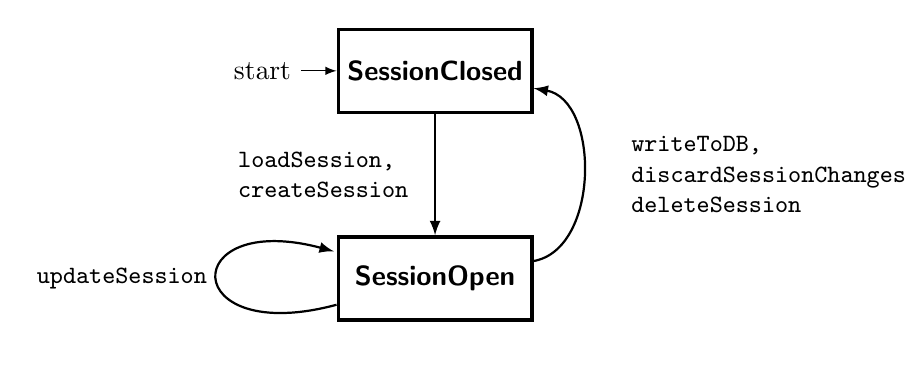
\begin{tikzpicture}[>=latex]
  \tikzstyle{state} = [draw, very thick, fill=white, rectangle, minimum height=3em, minimum width=7em, node distance=7.5em, font={\sffamily\bfseries}]
  
  \tikzstyle{stateEdgePortion} = [black,thick];
  \tikzstyle{stateEdge} = [stateEdgePortion,->];
  \tikzstyle{edgeLabel} = [pos=0.5, font={\sffamily\small}];

  \node[initial,state] (A)              {SessionClosed};
  \node[state]         (B) [below of=A] {SessionOpen};

  \path (A) edge[stateEdge]   node[edgeLabel, xshift=-1cm, text width=3cm] {\texttt{loadSession, createSession}} (B)
        (B) edge[stateEdge, bend right=80]   node[edgeLabel, xshift=6em, text width=3cm] {\texttt{writeToDB, discardSessionChanges, deleteSession}} (A)
            edge[stateEdge, loop left]   node[edgeLabel] {\texttt{updateSession}} (B);
\end{tikzpicture}
}
\caption{Session Handler Resource Usage Protocol}
\label{fig:sessionstates}
\end{figure}

Figure ~\ref{fig:sessionstates} shows the resource usage protocol associated
with the session handler, and Figure \ref{fig:sessioneffect} the corresponding
algebraic effect. In this application, there are two states:
In \texttt{SessionClosed}, the user may load or create a
session.
In \texttt{SessionOpen}, the user may update the
representation of the session in memory, serialise the session and write it to
the database, or delete the session and invalidate the user's session key. 
These two states ensure that changes are explicitly either
written or discarded, eliminating the possibility of a developer updating the
session but neglecting to commit it to persistent storage. This, of course, is
under the assumption that the process exits cleanly: we attempt to facilitate
this by writing total functions where possible.

Much like the SQLite effect, we encapsulate failure by reflecting it in the
resource associated with the effect. 

\begin{SaveVerbatim}{sstep}

data SessionStep = SessionClosed | SessionOpen
\end{SaveVerbatim}

\begin{SaveVerbatim}{sres}
data SessionRes : SessionStep -> Type where
  InvalidSession : SessionRes s  
  ValidSession   : SessionID -> 
                   SessionData -> 
                   SessionRes s

\end{SaveVerbatim}

\useverb{sstep}

\useverb{sres}

%The \texttt{SessionRes} data type is parameterised over the current state,
%which determines which operations may be performed, and has two constructors:
%\texttt{InvalidSession} and \texttt{ValidSession}. If an operation such as
%creating a new session fails, no further side-effecting calls will be made, in
%turn preserving integrity. 

% =================================================
\section{Type-aware form handling}

\label{form}
Programming web applications often involves processing user data, which may
then be used in further effectful computations. Data submitted using a form is
transmitted over the internet as a string as part of an HTTP request, which
traditionally involves losing associated type information.

This can in turn lead to risks; developers may assume that data is
of a certain type, and therefore discount the possibility that it may have been
modified by an attacker. One example would be the traversal of paginated data,
in which a form is used to make a request to retrieve the next page of data.
This may involve sending an integer detailing the current page, which could be
used in a query such as:

\begin{SaveVerbatim}{selectq}

'SELECT `name`, `address` FROM `staff` LIMIT ' + 
       page + ', 5';

\end{SaveVerbatim}
\useverb{selectq}

\noindent
The \texttt{page} variable is assumed to be an integer, but may instead be
modified by an attacker to include a malicious string which would alter the
semantics of the query, allowing an attacker to execute a blind SQL injection
attack. % Might be a good idea to cite an SQL injection paper which uses LIMIT
% clauses here

In this section, we present a mechanism by which we introduce a DSL
for the creation of web forms which preserve type information, implemented
as a dependent algebraic effect. Once the form has
been submitted, retrieved information is passed directly to a
developer-specified function for handling, without the need to manually check
and deserialise data. 

We begin with a simple example of a form which requests a user's name, and
echoes it back. Firstly, we define a form handler which echoes back a string
provided by the form handler. It has one argument of type \texttt{Maybe
String}, which accounts for the possibility that the user may have specified
incorrect data within the form.

\begin{SaveVerbatim}{sayhello}

sayHello : Maybe String -> 
           FormHandler [CGI (InitialisedCGI TaskRunning)]
sayHello (Just name) = output ("Hello, " ++ name ++ "!")
sayHello _ = output "Error!"

\end{SaveVerbatim}
\useverb{sayhello}

We then specify this in a list of handlers, detailing the arguments, available effects, handler function and unique identifier:

\begin{SaveVerbatim}{handerlist}

handlers : HandlerList
handlers = [handler args=[FormString], 
                    effects=[CgiEffect], 
                    fn=sayHello, 
                    name="sayHello"]

\end{SaveVerbatim}
\useverb{handerlist}

We also define a form to take in a name from the user, and specify that it should use the \texttt{sayHello} handler.

\begin{SaveVerbatim}{showhello}

showHelloForm : UserForm
showHelloForm = do
  addTextBox "Name" FormString Nothing
  useEffects [CgiEffect]
  addSubmit sayHello handlers

\end{SaveVerbatim}
\useverb{showhello}

\noindent
Finally, we specify that if data has been submitted for processing, then it
should be passed to the form handler. If not, then the form should be shown.

\begin{SaveVerbatim}{cgihello}

cgiHello : CGIProg [] ()
cgiHello = do
  handler_set <- isHandlerSet
  if handler_set then do
    handleForm handlers
    return ()
  else do
    addForm "nameform" "helloform" showHelloForm
    return ()

main : IO ()
main = runCGI [initCGIState] cgiHello

\end{SaveVerbatim}
\useverb{cgihello}

\noindent
When this CGI application is invoked, it will begin by outputting a form to the
page, requesting a name from the user. Upon submission of the form, the form
handler will be invoked, and the name will be used in the output.

In Sections ~\ref{formcons} and ~\ref{formhandling}, we examine implementation
of the form-handling system: namely, the effect which allows the creation of
forms, and the handling code which deserialises the data and passes it to the
user-specified handler function.  

\subsection{Form Construction}
\label{formcons}
Each form element is specified  to hold a particular type of data, which, assuming that the correct type of data is specified by the user, is passed directly to the handler function. In order to encapsulate this, we firstly define the allowed data types as part of an algebraic data type, \texttt{FormTy}.

\begin{SaveVerbatim}{formty}

data FormTy = FormString | FormInt
            | FormBool   | FormFloat
            | FormList FormTy 

\end{SaveVerbatim}
\useverb{formty}

\noindent
Since types in \idris{} are first-class, we may use this to convert
between abstract and concrete representations of allowed form types:

\begin{SaveVerbatim}{interpformty}

interpFormTy : FormTy -> Type
interpFormTy FormString = String
interpFormTy FormInt = Int
interpFormTy FormBool = Bool
interpFormTy FormFloat = Float
interpFormTy (FormList a) = List (interpFormTy a)

\end{SaveVerbatim}
\useverb{interpformty}

\begin{SaveVerbatim}{formeff}
using (G : List FormTy, E : List WebEffect)
  data FormRes : List FormTy -> List WebEffect -> Type where
    FR : Nat -> List FormTy -> List WebEffect -> String -> FormRes G E
  
  data Form : Effect where
    AddTextBox      : (label : String) -> (fty : FormTy) -> (Maybe (interpFormTy fty)) -> 
                      Form (FormRes G E) (FormRes (fty :: G) E) () 
    AddSelectionBox : (label : String) -> (fty : FormTy) -> (vals : Vect m (interpFormTy fty)) -> 
                      (names : Vect m String) ->
                      Form (FormRes G E)  (FormRes (fty :: G) E) ()
    AddRadioGroup   : (label : String) -> (fty : FormTy) -> (vals : Vect m (interpFormTy fty)) ->
                      (names : Vect m String) -> (default : Int) ->
                      Form (FormRes G E)  (FormRes (fty :: G) E) ()
    AddCheckBoxes   : (label : String) -> (fty : FormTy) -> (vals : Vect m (interpFormTy fty)) ->
                      (names : Vect m String) -> (checked_boxes : Vect m Bool) ->
                      Form (FormRes G E)  (FormRes ((FormList fty) :: G) E) ()
    Submit          : (mkHandlerFn ((reverse G), E)) -> String -> 
                      Form (FormRes G E)  (FormRes [] [])       String
\end{SaveVerbatim}

\begin{figure*}[t]
\begin{center}
\useverb{formeff}
\end{center}
\caption{Form Effect}
\label{fig:formeffect}
\end{figure*}

In order to specify a form, we once again use \texttt{Effects}. By recording
the type of each form element as it is added in the type of the form, we may
statically ensure that the user-supplied handler function is of the correct
type to handle the data supplied by the form: the specification of an
incompatible handler will result in a compile-time type error. The \texttt{Form}
effect and associated resource \texttt{FormRes} is given in Figure 
\ref{fig:formeffect}.
The \texttt{using} notation here indicates that within
the block, where \texttt{G} and \texttt{E} occur they are implicit arguments with
the given type.

The general process of form construction is illustrated by the \texttt{AddTextBox}
and \texttt{Submit} operations of the \texttt{Form} effect:

\begin{SaveVerbatim}{formeffsmall}

data Form : Effect where
  AddTextBox : (label : String) -> (fty : FormTy) -> 
               Maybe (interpFormTy fty) -> 
               Form (FormRes G E) 
                    (FormRes (fty :: G) E) () 
     ...
  Submit : (mkHandlerFn ((reverse G), E)) -> String -> 
           Form (FormRes G E) (FormRes [] []) String

\end{SaveVerbatim}
\useverb{formeffsmall}

\noindent
These make use of the resource associated with the effect, \texttt{FormRes}, to
construct the form. Adding a field such as a text box adds a new type, \texttt{fty}
to the list of field types, carried in the resource. When the form is complete,
the \texttt{Submit} operation adds a submit button and returns the
HTML text for the form, flushing the list of field
types, and using it to construct the type for an appropriate handler function.
%
To specify a form instance, we define a function of type \texttt{UserForm}:

\begin{SaveVerbatim}{userform}

UserForm : Type
UserForm = EffM m [FORM (FormRes []) 
                        (FormRes [])] String

\end{SaveVerbatim}
\useverb{userform}

\noindent
All forms are required to include a submit button, as mandated by the
requirement that 

The input and output resource contains an empty list of types, which means that
any form which includes fields must also include a submit button. Adding fields
adds to the list of types, and only adding a submit button empties that list.
Note that there is no need to restrict this effect to running in the \texttt{IO}
monad since creating a form merely returns HTML text, with no side-effects by
default.

Handlers may only be associated with a form if they have argument types
corresponding to the types associated with the form elements. Additionally, we
wish to name the function in order for it to be serialised, whilst requiring a
proof that the specified name is associated with the function. If this were not
the case, it would be possible to specify a function which satisfies the type
requirement, without guaranteeing that it the serialised data corresponded to
that function, thus rendering the check pointless. 

Before associating a handler function with the form, we must specify the
effects available to the handler. This is done through the use of the
\texttt{useEffects}, which updates the list of effects in the type of the form
resource. By doing this, we may subsequently use the effects in calculations at
the type level, in particular when calculating the type of the handler function
for the form. 

\begin{SaveVerbatim}{useeffs}

useEffects : (effs : List WebEffect) ->
             EffM m [FORM (FormRes G E)] 
                    [FORM (FormRes G effs)] ()
useEffects effs = (UseEffects effs)

\end{SaveVerbatim}
\useverb{useeffs}

\noindent
A \texttt{WebEffect} is an effect which is usable in a web application, and can
be converted to an \texttt{EFFECT} using:

\begin{SaveVerbatim}{interpwebeff}

webEffect : WebEffect -> EFFECT

\end{SaveVerbatim}
\useverb{interpwebeff}

Whilst it is not possible to serialise arbitrary effects due to the associated
difficulties with serialising initial resource environments, we allow for three
effects to be serialised: \texttt{CGI}, \texttt{SQLITE} and \texttt{SESSION}.
This is, however, not an inherent limitation as the \texttt{Effects} library
permits introduction of additional effects within an effectful computation.
%
We may specify a handler function of type \texttt{FormHandler}:

\begin{SaveVerbatim}{formhandler}

FormHandler : List EFFECT -> Type
FormHandler effs = Eff IO effs ()

\end{SaveVerbatim}
\useverb{formhandler}

\noindent
In order to associate a handler with a form, we may call the \texttt{addSubmit}
function:

\begin{SaveVerbatim}{addsubmit}

addSubmit : (f :  mkHandlerFn ((reverse G), E)) ->
            (fns : HandlerList) ->
            {default tactics 
              { applyTactic findFn 100; solve; }
              prf : FnElem f fns} ->
            EffM m [FORM (FormRes G E)]
                   [FORM (FormRes [] [])] 
                   String
addSubmit f handlers {prf} = (Submit f name)
    where name : String
          name = getString' f handlers prf          

\end{SaveVerbatim}
\useverb{addsubmit}

\noindent
This function takes a handler function and a list of available handlers, along with
an automatically constructed proof (using the a \texttt{default} argument) that the
handler is available.
Let us look at each aspect of this function in turn. Firstly, the
\texttt{mkHandlerFn} function calculates the required type of the handler
function from the list of types associated with the form elements, and the
effects we specified with \texttt{useEffects}. Note that since we prepend types
to the list of \texttt{FormTy}s as opposed to appending them, we must reverse
the list.

\begin{SaveVerbatim}{mkhandlerfnty}

MkHandlerFnTy : Type
MkHandlerFnTy = (List FormTy, List WebEffect)

\end{SaveVerbatim}

\begin{SaveVerbatim}{mkhandlerfn}

mkHandlerFn' : List FormTy -> List WebEffect -> Type
mkHandlerFn' [] effs = FormHandler (map webEffect effs) 
mkHandlerFn' (x :: xs) effs = Maybe (interpFormTy x) -> 
                              mkHandlerFn' xs effs 

mkHandlerFn : MkHandlerFnTy -> Type 
mkHandlerFn (tys, effs) = mkHandlerFn' tys effs 

\end{SaveVerbatim}

\useverb{mkhandlerfnty}

\useverb{mkhandlerfn}

\noindent
The \texttt{mkHandlerFn} function takes a tuple describing the arguments and
web effects available to the handler function. When constructing the function
type, we encase all arguments withing \texttt{Maybe} type, in order to handle
failure should the supplied data fail to parse to the specified type.
%
To store a reference to a handler function, we use the \texttt{HandlerFn} type:

\begin{SaveVerbatim}{handlerfn}

HandlerFn : Type
HandlerFn = (ft ** (mkHandlerFn ft, String))

\end{SaveVerbatim}
\useverb{handlerfn}

\noindent
The \texttt{**} notation denotes a dependent pair, where the type of the second
element of the pair is parameterised over the value of the first element. It is
an existential binding;
the notation \texttt{(x ** P x)} can be read as ``there exists an \texttt{x} such that 
\texttt{P x} holds''.
Therefore a \texttt{HandlerFn} states that there exists a function type
\texttt{ft} such that we have a handler for it, and a unique string identifier
which is used to serialise a
reference to the handler function. 

In order to abstract away from this implementation detail, we make use of
\idris{} syntax rewriting rules. This allows us to define the following syntax
rewrite rule:

\noindent
\begin{SaveVerbatim}{syntaxhandler}

syntax 
  "handler args=" [args] ", effects=" [effs] ", fn=" [fn] 
  ", name=" [name] = ((args, effs) ** (fn, name))

\end{SaveVerbatim}
\useverb{syntaxhandler}

\noindent
We may then define handlers in a more intuitive fashion, without being
concerned with the implementation details. This allows us to write a handler
with one String argument, making use of the CGI effect, associated with the
\texttt{sayHello} handler function as follows:

\begin{SaveVerbatim}{handlerex}

handler args=[FormString], 
        effects=[CgiEffect], 
        fn=sayHello, 
        name="sayHello"

\end{SaveVerbatim}
\useverb{handlerex}

\noindent
We then store each \texttt{HandlerFn} in a \texttt{HandlerList}.

\begin{SaveVerbatim}{handlerlist}

HandlerList : Type
HandlerList = List HandlerFn

\end{SaveVerbatim}
\useverb{handlerlist}

To enforce the requirement that a supplied handler function must reside in the
list of available handlers, and therefore allow us to retrieve the name with
which to serialise the handler, we require a \textit{list membership proof},
\texttt{FnElem f fns}, which statically guarantees that a given item resides in
a list.

\begin{SaveVerbatim}{fnelem}

using (xs : HanderList , f : mkHandler (reverse G, E))
  data FnElem : mkHandlerFn ((reverse G), E) -> 
                HandlerList -> Type where
       FnHere  : FnElem f (((reverse G, E) ** 
                                  (f, fStr)) :: xs)
       FnThere : FnElem f xs -> FnElem f (x :: xs)

\end{SaveVerbatim}
\useverb{fnelem}

\noindent
\texttt{FnElem} is parameterised over \texttt{G} and \text{E}, the types of the
form elements and the effects used by the handler function. \texttt{FnHere}
is a proof that the element is at the head of the current point of the list,
whereas \texttt{FnThere} is a proof that the element is in the tail of 
the list. 
%TODO: this should probably be rewritten
We then use a simple automated proof search to
automatically generate the proof at compile time, should one exist. The proof
may then be used in subsequent computations: in our case, we use it to retrieve
the unique identifier for the function. If the automated proof search fails,
compilation will fail.

Finally, we serialise the argument types, supported effects, and return
type of the handler, to allow the form data to be 
deserialised and ensure that the correct handler is executed on the
server. 

Although sending details of the handler function to the client may appear to be
a security risk, we envisage that the use of symmetric encryption or a
cryptographic nonce would alleviate this. Ultimately, we hope to implement a
web server with persistent state, which would eliminate the need for
serialisation altogether.

Running form construction is achieved as an operation of the CGI
effect, \texttt{AddForm}, which then outputs the generated HTML to the page.
The generated metadata describing the handler function is serialised as a
hidden HTML field.

\subsection{Form Handling}
\label{formhandling}
Once the form has been submitted, a web application may handle the submitted
data by invoking \texttt{HandleForm}. This will check for the
existence of the hidden \texttt{handler} field, which contains the previously
serialised metadata about the form handler, before deserialising the
data into a \texttt{MkHandlerFnTy}. 

With this data, we then look up the function in the list of registered
handlers by using the unique handler identifier. In order to apply
the handler function to the data submitted in the form, we must first prove to
the type checker that the deserialised \texttt{MkHandlerFnTy} is the same as
the one retrieved from the list of registered handlers. We do this by making
use of the \texttt{decEq} function, which determines whether two types are
equal, returning a proof of equality if so, and a proof of inequality if not.

\begin{SaveVerbatim}{deceqty}

decEq : DecEq t => (x : t) -> (y : t) -> Dec (x1 = x2)

\end{SaveVerbatim}
\useverb{deceqty}

We then use the \texttt{with} construct, inspired by
\textit{views} in Epigram \cite{mcbride.mckinna:viewfromleft}, to rewrite the
arguments on the left hand side. This allows us to construct a function which,
given the stored handler, the data required to
construct the function type and the \texttt{MkHandlerFnTy} deserialised from
the form, determines whether the two \texttt{MkHandlerFnTy}s are decidably
equal. If so, we rewrite this on the left hand side since the equality proof
demonstrates that the recorded function may also be used to handle the form
data. If not, the computation fails.

\begin{SaveVerbatim}{checkfunctionsty}

checkFunctions : (reg_fn_ty : MkHandlerFnTy) -> 
                 (frm_fn_ty : MkHandlerFnTy) -> 
                 mkHandlerFn reg_fn_ty -> 
                 Maybe (mkHandlerFn frm_fn_ty)
\end{SaveVerbatim}

\begin{SaveVerbatim}{checkfunctions}
checkFunctions reg_ty frm_ty reg_fn with 
                             (decEq reg_ty frm_ty)
  checkFunctions frm_ty frm_ty reg_fn 
                        | Yes refl = Just reg_fn
  checkFunctions reg_ty frm_ty reg_fn 
                        | No _ = Nothing

\end{SaveVerbatim}

\useverb{checkfunctionsty}

\useverb{checkfunctions}

\noindent
We may then parse the arguments according to the types specified by the handler
function, and then apply the arguments to the handler function through the use
of partial application. Finally, we may run the handler function, ensuring that
all updates made to the CGI state are propagated.

%-----------------------------
%-----------------------------
\section{Extended Example: Message Board}
\label{messageboard}
In this section we consider a larger example---a message board application
which allows users to register, log in, view and create threads, and list and
create new posts in threads. 

Firstly, we create a database schema in which to record information stored by
the message board. We create three tables: \texttt{Users}, which contains a
unique User ID, usernames and passwords; \texttt{Threads}, which contains a
unique thread ID, a title, and the ID of the user who created the thread; and
\texttt{Posts}, which contains a unique post ID, the ID of the thread to which
each post belongs, the content of the post, and the ID of the user that created
the post.

Secondly, we use a \texttt{GET} variable, \texttt{action}, to indicate which page of the
message board should be displayed, and pattern-match on these to call the
appropriate function which displays the page. Some pages, such as the page
which shows all of the posts in a thread, require a second argument,
\texttt{thread\_id}.  

\subsection{Handling requests}
The entry point to any CGI application is the \texttt{main} function. From
here, we run the remainder of the program through a call to \texttt{runCGI},
which we initialise with empty initial environments for the \texttt{CGI}, 
\texttt{Session} and
\texttt{SQLite} effects, so they may be used in further computations. 

\begin{SaveVerbatim}{msgmain}

main : IO ()
main = do (runCGI [initCGIState, 
                  InvalidSession, ()] 
           handleRequest)
          return ()

\end{SaveVerbatim}
\useverb{msgmain}

\noindent
We define a function, \texttt{handleRequest}, which firstly determines
whether submitted form data must be handled, by checking whether a handler
variable exists.
If so, then the form handling routine is called, which executes the
corresponding handler function as specified in Section ~\ref{formhandling}. If
not, then the \texttt{handleNonFormRequest} function is called, which inspects
the \texttt{GET} variables in order to display the correct page.

\begin{SaveVerbatim}{handlereq}

handleRequest : CGIProg 
     [SESSION (SessionRes SessionUninitialised), 
      SQLITE ()] ()
handleRequest = do 
  handler_set <- isHandlerSet
  if handler_set then do
    lift' (handleForm handlers)
    Effects.return ()
  else do
    action <- lift' (queryGetVar "action")
    thread_id <- lift' (queryGetVar "thread_id")
    handleNonFormRequest action (map strToInt thread_id)

\end{SaveVerbatim}
\useverb{handlereq}

\subsection{Thread Creation}
We create four forms: one to handle registration, one to handle logging in,
one to handle the creation of new threads, and one to handle the creation of
new posts. For example, the form used to create a new thread
contains elements for the title of the new thread and the content of the
first post of the new thread:

\begin{SaveVerbatim}{newthread}

newThreadForm : UserForm
newThreadForm = do
  addTextBox "Title" FormString Nothing
  addTextBox "Post Content" FormString Nothing 
  useEffects [CgiEffect, SessionEffect, SqliteEffect]
  addSubmit handleNewThread handlers

\end{SaveVerbatim}
\useverb{newthread}

\noindent
This consists of two text boxes: one for the title of the thread, and one
for the content of the first post. Both are of type \texttt{String}, as denoted
by the \texttt{FormString} argument, and both have no default value. The
handler function may make use of the \texttt{CGI}, \texttt{SESSION} and
\texttt{SQLITE} effects, and the handler function is specified as
\texttt{handleNewThread}. The \texttt{handlers} argument refers to the list of
form handlers, and is of the following form:

\begin{SaveVerbatim}{msghandlers}

handlers : HandlerList
handlers = [
 (handler args=[FormString, FormString], 
          effects=[CgiEffect, SessionEffect, SqliteEffect], 
          fn=handleRegisterForm, 
          name="handleRegisterForm"),
  
 (handler args=[FormString, FormString], 
          effects=[CgiEffect, SessionEffect, SqliteEffect], 
          fn=handleNewThread, 
          name="handleNewThread"),
     ...]

\end{SaveVerbatim}
\noindent
\useverb{msghandlers}

\noindent
Creating a new thread (shown in Figure \ref{fig:handlethread})
requires a user to be logged in, so that the thread
starter may be recorded in the database. In order to do this, we make use of
the session handler. We define a function \texttt{withSession}, which attempts
to retrieve the session associated with the current request, and if it exists,
executes a function which is passed the associated session data. If not, then a
failure function is called instead. Should the form handler function be called
with invalid arguments, an error is shown.

\begin{SaveVerbatim}{handlenewthread}
handleNewThread : 
  Maybe String -> Maybe String -> 
  FormHandler [CGI (InitialisedCGI TaskRunning), 
               SESSION (SessionRes SessionUninitialised), 
               SQLITE ()]  
handleNewThread (Just title) (Just content) = do 
  withSession (addNewThread title content) notLoggedIn
  return ()
handleNewThread _ _ = do 
  outputWithPreamble "<h1>Error</h1><br />There was 
       an error posting your thread."
  return ()
\end{SaveVerbatim}

\begin{figure}[h]
\useverb{handlenewthread}
\caption{Thread Creation}
\label{fig:handlethread}
\end{figure}

\noindent
Once we have loaded the session data from the database, we then check whether
the \texttt{UserID} variable is set, which demonstrates that a user has
successfully logged into the system, and allows us to use the ID in subsequent
computations. The database operation to insert the thread into the database is
performed by \texttt{threadInsert}, shown in Figure \ref{fig:threadins}.
This uses a library function \texttt{executeInsert}, which abstracts over the
low-level resource usage protocol, enabling for provably-correct database
access without the excess boilerplate code. In addition, \texttt{executeInsert}
returns the unique row ID of the last item which was inserted, which may be
used in subsequent computations. In the case of the message board, we use this
to associate the first post of the thread with the thread being inserted.

\begin{SaveVerbatim}{threadins}
threadInsert : Int -> String -> String -> 
               Eff IO [SQLITE ()] Bool
threadInsert uid title content = do
  let query = "INSERT INTO `Threads` 
    (`UserID`, `Title`) VALUES (?, ?)"
  insert_res <- (executeInsert DB_NAME query 
    [(1, DBInt uid), (2, DBText title)]
  case insert_res of
    Left err => return False
    Right thread_id => postInsert uid thread_id content
\end{SaveVerbatim}

\begin{figure}[h]
\useverb{threadins}
\caption{Thread Insertion}
\label{fig:threadins}
\end{figure}

\subsection{Listing Threads}

Listing the threads in the database is achieved using 
\texttt{executeSelect}, which returns either a
\texttt{ResultSet} or an error:

\begin{SaveVerbatim}{getthreads}

getThreads : Eff IO [SQLITE ()] (Either String ResultSet)
getThreads = 
    executeSelect DB_NAME query [] collectThreadResults
 where query = "SELECT `ThreadID`, `Title`, `UserID`, 
         `Username` FROM `Threads` NATURAL JOIN `Users`"

\end{SaveVerbatim}
\noindent
\useverb{getthreads}

\noindent 
Once the result set has been retrieved, we may iterate through the
results and output them to the page, including a link to a page which shows the
posts associated with the thread. This is shown in Figure \ref{fig:traverse}.
Since we know the structure of the returned
row from designing the query, we may pattern match on each returned row to make
use of the returned values.

\begin{SaveVerbatim}{traversethreads}
traverseThreads : ResultSet -> 
  Eff IO [CGI (InitialisedCGI TaskRunning)] ()
traverseThreads [] = return ()
traverseThreads (x::xs) = do traverseRow x
                             traverseThreads xs
  where traverseRow : List DBVal -> 
           Eff IO [CGI (InitialisedCGI TaskRunning)] ()
        traverseRow ((DBInt thread_id)::
                     (DBText title)::
                     (DBInt user_id)::
                     (DBText username)::[]) =
           (output $ "<tr><td>
            <a href=\"?action=showthread&thread_id=" ++ 
            (show thread_id) ++ "\">" ++ 
            title ++ "</a></td><td>" ++ 
            username ++ "</td></tr>") 
        traverseRow _ = return ()
\end{SaveVerbatim}

\begin{figure}[h]
\useverb{traversethreads}
\caption{Thread Insertion}
\label{fig:traverse}
\end{figure}

\subsection{Authentication}

Once a user submits the login form, the associated handler queries the database
to ascertain whether a user with the given username and password exists through
a call to the \texttt{authUser} function. This is shown in Figure
\ref{fig:handlelogin}. If so, then the session handler is
invoked, and a session is initialised with the user ID retrieved from the
database. The session ID is then set as a cookie using the CGI effect, so that
it may be used in subsequent requests. Any failures, for example with creating
a new session or querying the database, are reported to the user.

\begin{SaveVerbatim}{handlelogin}
handleLoginForm (Just name) (Just pwd) = do
  auth_res <- lift' (authUser name pwd)
  case auth_res of
    Right (Just uid) => do
      set_sess_res <- setSession uid
      if set_sess_res then do
        lift' (output $ "Welcome, " ++ name)
        return ()
      else do
        lift' (output "Could not set session")
         return ()
    Right Nothing => do
      lift' (output "Invalid username or password")
      return ()
    Left err => do
      lift' (output $ "Error: " ++ err)
      return ()
\end{SaveVerbatim}

\begin{figure}[h]
\useverb{handlelogin}
\caption{Thread Insertion}
\label{fig:handlelogin}
\end{figure}

Implementations for the insertion and display of posts, alongside registration,
follow the same structure.

Although we have described a relatively simple application, we have shown that
through the use of embedded domain-specific languages, 
and particularly by encapsulating resource usage protocols in the types,
we can write verified
code that fails to compile should resources be incorrectly accessed.
Additionally, we have used the form handling mechanism to simply handle the
arguments passed by the user. Importantly, we have shown that dependent types
can be used to increase confidence in an (albeit simplified) real-world
application, without requiring developers to supply proofs or indeed work
explicitly with dependent types. 

%-----------------------------
%-----------------------------
\section{Related Work}
\citet{meijer:cgi} implemented a CGI library which was among the first
libraries to handle web scripting monadically, and allows the user to implement
application logic without having to consider the low-level details such as
parsing in CGI data from the environment, or printing headers to the remote
browser. The library also provides support for cookies and basic form handling. 

\citet{thiemann:wash} adds the notion of a CGI Session for maintaining
state, and provides more sophisticated form-handling methods. In particular,
callbacks may be associated with submit buttons, with nameless representations
for form inputs. Both implementations of the CGI library,
being built upon monads, mean that the use of additional effects such as
database access is achieved either through monad transformers or 
performing arbitrary IO operations. Both of these approaches are limited---the
former does not scale well to multiple effects, and the latter allows for the
introduction of errors by allowing the violation of resource usage protocols.

\citet{plasmeijer:idata} describe an alternative approach to type-safe form
handling through the
\textit{i}nteractive \textit{Data}, or \idata{} abstraction. Instead of
processing being triggered by form submission, as in the approach described in
this paper, applications created in the \idata{} toolkit are 
edit-driven. This means that upon a component being edited, a computation
occurs, given the state of the current form. Should a user enter invalid data, for example by entering
text in a field designated for integers, the change will be reverted. This is
demonstrated practically through the use of \idata{} to implement a conference
management system \cite{plasmeijer:cms}.

The concept of \idata{} is taken further by the introduction of \itasks{}
\cite{plasmeijer:itasks}, which make use of a workflow system to allow multiple
\idata{} forms to interact with one another. This is achieved using
high-level combinators which allow the implementation of concepts such as
recursion, sequence and choice in a scalable fashion.

Ur\/Web \cite{urweb} is a library built for the Ur language, which does not use
full dependent types but does have an expressive type system with 
record types and type-level computation.  By using these concepts,
Ur\/Web may generate provably correct and unexploitable DOM code and SQL
queries from records, without requiring developers to supply proofs.  In
contrast to using runtime code generation, which is prone to obscure code
generation errors, Ur\/Web makes use of its static type system to guarantee
that metaprograms---in this case, generated SQL and DOM code---must be correct
and secure.  Such ideas regarding the use of static checking of metaprogram
generation will be extremely useful when considering an object-relational
mapping system, which we hope to implement in the near future. It will also be
interesting to see how such concepts may be applied with a yet more expressive
type system involving full dependent types.

Formlets \cite{cooper:formlets} are a well-known functional abstraction over web forms, making use of McBride and Paterson's applicative functors \cite{mcbride:applicative} to provide an extensible and powerful method of building and handling web forms. 
Our approach differs in that we check that handler functions conform to the types of the elements in the forms by parameterising the resource associated with the form construction effect, as opposed to using a preprocessor to rewrite the form elements in applicative notation.
Our framework does not yet support composition of sections of forms, as is the case with formlets, but we foresee no problems with extending our DSL to add this functionality.

Ensuring conformance to resource usage protocols has been attempted using the
notion of \emph{typestate} in object-oriented languages
\cite{deline:typestates}. Our approach differs in that we make no changes to
the type system in order to implement this functionality; we check resource
usage protocol conformance directly within \idris{}.  Additionally, our
handler-based approach gives greater control over side effects.

Java is often used as a language to write enterprise-level web applications. Frameworks such as the Java Persistence API (JPA) \cite{jpa} use Java annotations to translate data models into the appropriate database schemata, but such code may soon become unwieldy due to the large amount of redundant boilerplate code such as accessor and mutator functions. WebDSL \cite{webdsl} is a domain-specific language written primarily to
introduce new abstractions which aim to reduce the amount of boilerplate code
that must be written and maintained by developers. 
The DSL is parsed into an abstract syntax tree, modified using rewrite rules, and elaborated back into Java code. 
%WebDSL also applies similar concepts to implement a \textit{template system} for the presentation of data entities. We look to
%implement many of these ideas, but as effects within the IdrisWeb
%framework, as with the form construction effect.

%-----------------------------
%-----------------------------

\section{Conclusions}

Dependently-typed languages promise to support machine checkable program
correctness proofs, but to date they have remained relatively unused for
practical purposes. By using embedded domain-specific languages, we can
abstract away some of the complexities of creating correctness proofs and
provide expressive libraries, giving guarantees by the successful compilation
of a program (assuming the use of specific enough types) without additional
proofs.

Our framework provides several static
guarantees. Data submitted by users is inherently unsafe and
means systems are vulnerable to attacks
such as SQL injection. This particular threat is ameliorated due
to elements being associated with specific types during form construction. This
immediately eliminates the possibilities of SQL injection attacks on non-string
types. Since failures are handled transparently, no runtime errors are written
to the browser, meaning that attackers may not use such information to aid
attacks. Additionally, since checking is performed on the types of the form
elements and the types of arguments accepted by the handler, it is impossible
to associate a form with a handler incompatible with the submitted data.

Many external libraries also follow (unchecked or dynamically checked) 
resource usage protocols.
Incorrect usage is however still possible, for
example by forgetting to release acquired resources or failing to
initialise a library correctly. By creating high-level bindings to these
libraries, however, we may statically enforce these resource-usage protocols,
ensuring that the libraries are used correctly. Whilst previous work has
demonstrated that this is possible through the use of embedded DSLs
\cite{brady:edsl} and dependent algebraic effects \cite{brady:effects},
this paper has provided more substantial examples of real-world applications. 

In particular, the framework guarantees that it is not possible for a CGI 
application to
produce an internal server error due to content being written to the remote
host prior to headers. With regard to database access, we may statically
guarantee that library calls are made in the correct order, and calls to
retrieve rows of data are made only when more data is available. Additionally, by encoding desired invariants within operation types, we may gain static guarantees about adherence to resource usage protocols and failure handling.
Enforcing resource usage protocols also guards against common programmer
errors, saving debugging time by identifying errors at compile time.

\subsection{Further Work}

We have shown that embedded domain-specific languages using dependent types and
algebraic effects can be used to increase confidence in web applications, but much more
can be done using the same approach.

There are many other applications which make use of specific resource usage
protocols, for example popular cryptography libraries such as
\textit{Sodium}\footnote{\texttt{https://github.com/jedisct1/libsodium}}.
Applying a similar approach would allow for sensitive programs requiring
cryptographic routines to be written using a language with full dependent
types, in turn adding an extra layer of confidence in their security. 

Whilst the use of CGI allows for experimenting with the use of dependent types
in a real-world scenario such as web programming, there remain practical
considerations about its scalability, as a separate process must be created for
each individual request. We believe that the use of FastCGI may alleviate this,
but ultimately, we would like to create a web server written in \idris{}, which
would make more efficient usage of resources. 

Since at this stage we have concentrated on the use of dependent types for
enforcing resource usage protocols and type-safe form handling, we currently
handle the generation of HTML in an unstructured manner. Future work will
entail a DOM library to facilitate the generation and manipulation of HTML, in
turn giving stronger guarantees about its correctness. Other planned features
include a template system, allowing for web pages to be automatically generated
from data, and an object-relational mapping system. 
It would also be interesting to 
explore the use of continuation-passing approaches \cite{queinnec:ioc} to enhance the usability of the framework.

Type providers, as originally implemented in F\# \cite{msr:tp}, allow external data sources to be used to import
external information to be used during compilation. 
In this way, it becomes possible to use the extra type
information to statically ensure the validity of artefacts such as SQL
queries and data structures. If data structures within the program do not
conform to a given database schema, for example, then the program will not
type-check.  Type providers have been implemented for 
\idris{} 
\cite{christiansen:dtp}, exploiting the fact that types can be
calculated by functions to avoid unsafely generating extra code in the type provider
step. We believe that this technique would be an interesting avenue of exploration to provide further static guarantees about the form of database queries.

Dependently-typed languages provide great promise for the construction of
secure and correct programs. Through the use of embedded domain-specific
languages, we hope that more developers may benefit from the extra guarantees
afforded by dependent types, resulting in more stable, secure applications.

% Cryptography bindings would be really good.
% Integration with a web server instead of doing everything over CGI
% Improvements to form handling system
% Less raw SQL, use get more type-safety by using more complex EDSLs for database access thus further minimising errors


%\appendix
%\section{Appendix Title}

%This is the text of the appendix, if you need one.

%-----------------------------
%-----------------------------

\acks
This work has been supported by the Scottish Informatics and Computer Science Alliance (SICSA) and the EPSRC. We would like to thank the contributors to the \idris{} language, especially the authors of the original \texttt{Network.Cgi} and \texttt{SQLite} libraries.
We are very grateful to Peter Thiemann and the anonymous reviewers for their insightful and constructive comments.
% SICSA / EPSRC (grant number?
% #idris
% Idris contributors, in particular Melissa for the SQLite bindings and whoever wrote Network.Cgi

% We recommend abbrvnat bibliography style.

\bibliographystyle{plainnat}

% The bibliography should be embedded for final submission.

\bibliography{refs}
%\begin{thebibliography}{}
%\softraggedright
%
%\bibitem[Smith et~al.(2009)Smith, Jones]{smith02}
%P. Q. Smith, and X. Y. Jones. ...reference text...
%
%\end{thebibliography}


\end{document}

%                       Revision History
%                       -------- -------
%  Date         Person  Ver.    Change
%  ----         ------  ----    ------

%  2013.06.29   TU      0.1--4  comments on permission/copyright notices